\documentclass[11pt,a4paper]{article}
\usepackage{lac2017}
\usepackage{graphicx}
\usepackage{listings}
\usepackage{courier}
\lstset{basicstyle=\footnotesize\ttfamily,breaklines=true}

\sloppy
\newenvironment{contentsmall}{\small}

\title{Impulse-Response- and CAD-Model-Based \\ Physical Modeling in Faust}

%see lac2015.sty for how to format multiple authors!
%\author
%{Pierre-Amaury GRUMIAUX${}^1$, Romain MICHON${}^2$,\\ 
%\textbf{Emilio GALLEGO ARIAS}${}^1$\textbf{, and Pierre JOUVELOT}${}^1$
%\\ ${}^1$MINES ParisTech, PSL Research University, France  
%\\ ${}^2$CCRMA, Stanford University, USA
%}

\author
{Pierre-Amaury Grumiaux, 
	\\\textbf{Emilio GALLEGO ARIAS,} 
	\\\textbf{Pierre JOUVELOT}
	\\ MINES ParisTech, PSL Research University
	\\ France 
	\And
	Romain MICHON
	\\ CCRMA, Stanford University
	\\ USA
}

\newcommand{\f}{\textsc{Faust}}

\begin{document}
\maketitle

\begin{abstract}
  \begin{contentsmall}
    We present a set of tools to quickly implement modal physical models in the \f{} programming language. Models can easily be generated from any impulse response or 3D graphical representation of a physical object.

    This system targets users with little knowledge in physical modeling and willing to use this type of synthesis technique in a musical context.
  \end{contentsmall}
\end{abstract}

\keywords{
\begin{contentsmall}
Physical Modeling Synthesis, Faust Language, Digital Signal Processing
\end{contentsmall}
}

\section{Introduction}

The \f{} programming language has proven to be well suited to implement physical models of musical instruments~\cite{Michon2011} using waveguides~\cite{Smith2010} and modal synthesis~\cite{Adrien1991}.

In this short paper, we present two Python scripts allowing to easily generate \f{} modal physical models: \texttt{ir2dsp.py} and \texttt{mesh2dsp.py}.
\begin{itemize}
\item 
\texttt{ir2dsp.py} takes an audio file containing an impulse response as its main argument and converts it into a \f{} file implementing the corresponding modal physical model.
\item
\texttt{mesh2dsp.py} outputs the same type of model but takes an \texttt{.stl}\footnote{STereoLithography.} file containing the specification of any 3D object designed with a CAD\footnote{Computer-Aided Design.} program as its main argument.
\end{itemize}
\f{} programs generated by \texttt{ir2dsp.py} and \texttt{mesh2dsp.py} are ready to use and can be compiled to any of the \f{} targets (standalone applications, plug-ins, etc.).

After briefly describing these two tools, we'll evaluate them and provide directions for future works.

\section{Faust Modal Physical Model}
\label{sec:model}

Any linear percussion instrument can be implemented using a bank of resonant bandpass filters~\cite{Smith2010}. Each filter implements one mode (a sine or cosine function) of the system and can be configured by providing three parameters: the frequency of the mode, its gain, and its resonance duration (\textit{T60}).

Such a filter can be easily implemented in \f{} using a biquad filter (\texttt{tf2}) and by computing its poles and zeros for a given frequency (\texttt{f}) and \textit{T60} (\texttt{t60}):

\begin{lstlisting}
  modeFilter(f,t60) = tf2(b0,b1,b2,a1,a2)
  with{
        b0 = 1;
	b1 = 0;
	b2 = -1;
	w = 2*PI*f/SR;
	r = pow(0.001,1/float(t60*SR));
	a1 = -2*r*cos(w);
	a2 = r^2;
  };
  mode(f,t60,gain) = 
        modeFilter(f,t60)*gain;
\end{lstlisting}

The \texttt{modeFilter} function can be easily applied in parallel in \f{} using the \texttt{par} operator to implement any modal physical model:

\begin{lstlisting}
  model = 
        _ <: 
        par(i,nModes,
            mode(freq(i),t60(i),gain(i)))
        :> _;
\end{lstlisting}

The \f{}-generated block diagram corresponding to this code, with \lstinline{nModes = 4}, \lstinline{freq(i) = 100*(i+1)}, and \lstinline{(t60(i),gain(i))} as successively (0,9,0.9), (0.8,0.9), (0.6,0.5) and (0.5,0.6), can be visualized in Figure~\ref{fig:modalModel}.

\begin{figure}[htbp]
 	\centering 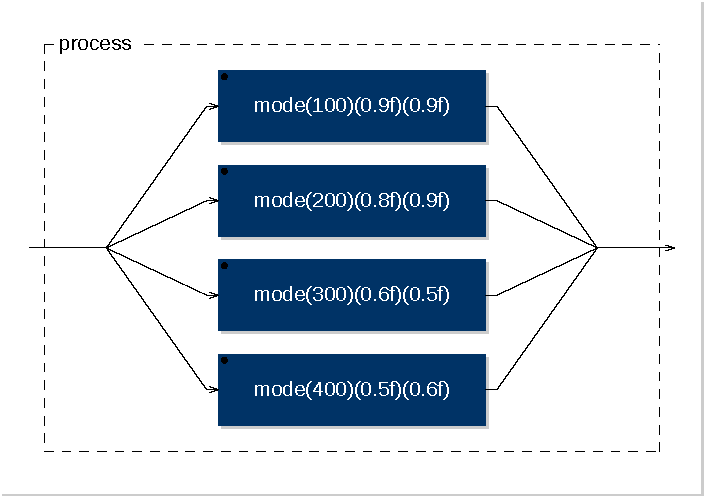
\includegraphics[width=\columnwidth]{pictures/modalModel}
	\caption{Block diagram of a \f{} modal physical model.}
	\label{fig:modalModel}
\end{figure}

This type of model can be easily excited by a filtered noise impulse (see Figure~\ref{fig:excitation}). The cutoff frequency of the lowpass and highpass filters can be used to excite specific zones of the spectrum of the model and to choose the ``excitation position.'' Since this system is linear, the same behavior could be achieved by scaling the gain of the different modes, but the filter approach that we use here will better integrate to our modular physical modeling synthesis toolkit, briefly presented in \S{}\ref{sec:future}. 

\begin{figure}[htbp]
 	\centering 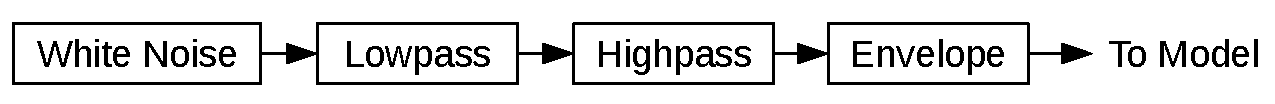
\includegraphics[width=\columnwidth]{pictures/excitation}
	\caption{Excitation generator algorithm used to drive our modal physical models.}
	\label{fig:excitation}
\end{figure}

\section{ir2dsp.py}
\label{sec:irdsp}

\texttt{ir2dsp.py} takes an audio file containing an impulse response as its main argument. After performing the Fast Fourier Transform (FFT) on it, modes information is extracted by carrying out peaks detection. The \textit{T60} of each mode is computed by measuring its bandwidth at -3 dB.

Modes information is formatted by \texttt{ir2dsp.py} to be plugged to a generic modal \f{} physical model similar to the one described in \S{}\ref{sec:model}. The output of the Python program is a ready-to-use \f{} file implementing the model. 

The goal of this tool is not to create very accurate models but rather to be able to strike any object (e.g., a glass, a metal bar, etc.), record the resulting sound, and turn it into a playable digital musical instrument.

\section{mesh2dsp.py}

The output of \texttt{mesh2dsp.py} is the same as \texttt{ir2dsp.py} (see \S{}\ref{sec:irdsp}), but it takes a \texttt{.stl} file as its input instead of an impulse response. \texttt{stl} is a common format supported by most CAD programs to export the description of 3D objects.

After converting the provided \texttt{.stl} file into a mesh, \texttt{mesh2dsp.py} performs a Finite Element Analysis (FEA) using Elmer (\texttt{https://www.csc.fi/web/elmer}, URL verified on 02/08/17. Git repository can be found at \texttt{https://github.com/ElmerCSC/elmerfem}.) Various parameters such as the Young Modulus, the Poisson Coefficient, and the density of the material of the object must be provided to carry out this task.

The result of the analysis is a set of eigenvalues and mass participations for each mode. Eigenvalues are then converted to mode frequencies and mass participations to mode gains. Unfortunately, this technique doesn't allow to calculate the \textit{T60} of the modes which can be configured by the user directly from the \f{} program. 

\section{Evaluation}

To evaluate the accuracy of \texttt{ir2dsp.py}, we recorded the impulse response of a can and generated its corresponding modal physical model. Figure~\ref{fig:spectro1} shows the spectrogram of the impulse response of the can and Figure~\ref{fig:spectro2} the spectrogram of the impulse response of the physical model generated by \texttt{ir2dsp.py}. \texttt{ir2dsp.py} was configured to detect peaks at a minimum value of -20 dB and at least 100 Hz spaced from each other. We see that the synthesized sound is pretty close to the recorded version. \textit{T60}s are not perfectly accurate since they were calculated by measuring the bandwidth of the mode. Tracking their evolution in the time domain would provide better results; thus we plan to use this technique in the future instead.

\begin{figure}[htbp]
  \centering
  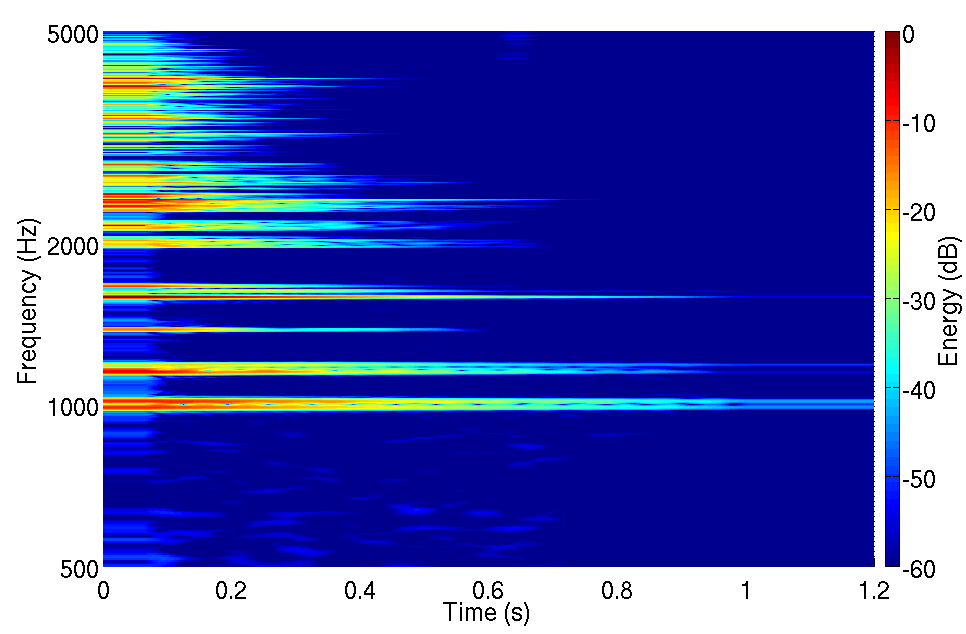
\includegraphics[width=\columnwidth]{pictures/canIR}
  \caption{Spectrogram of an impulse response of a can}
  \label{fig:spectro1}
\end{figure}

\begin{figure}[htbp]
  \centering
  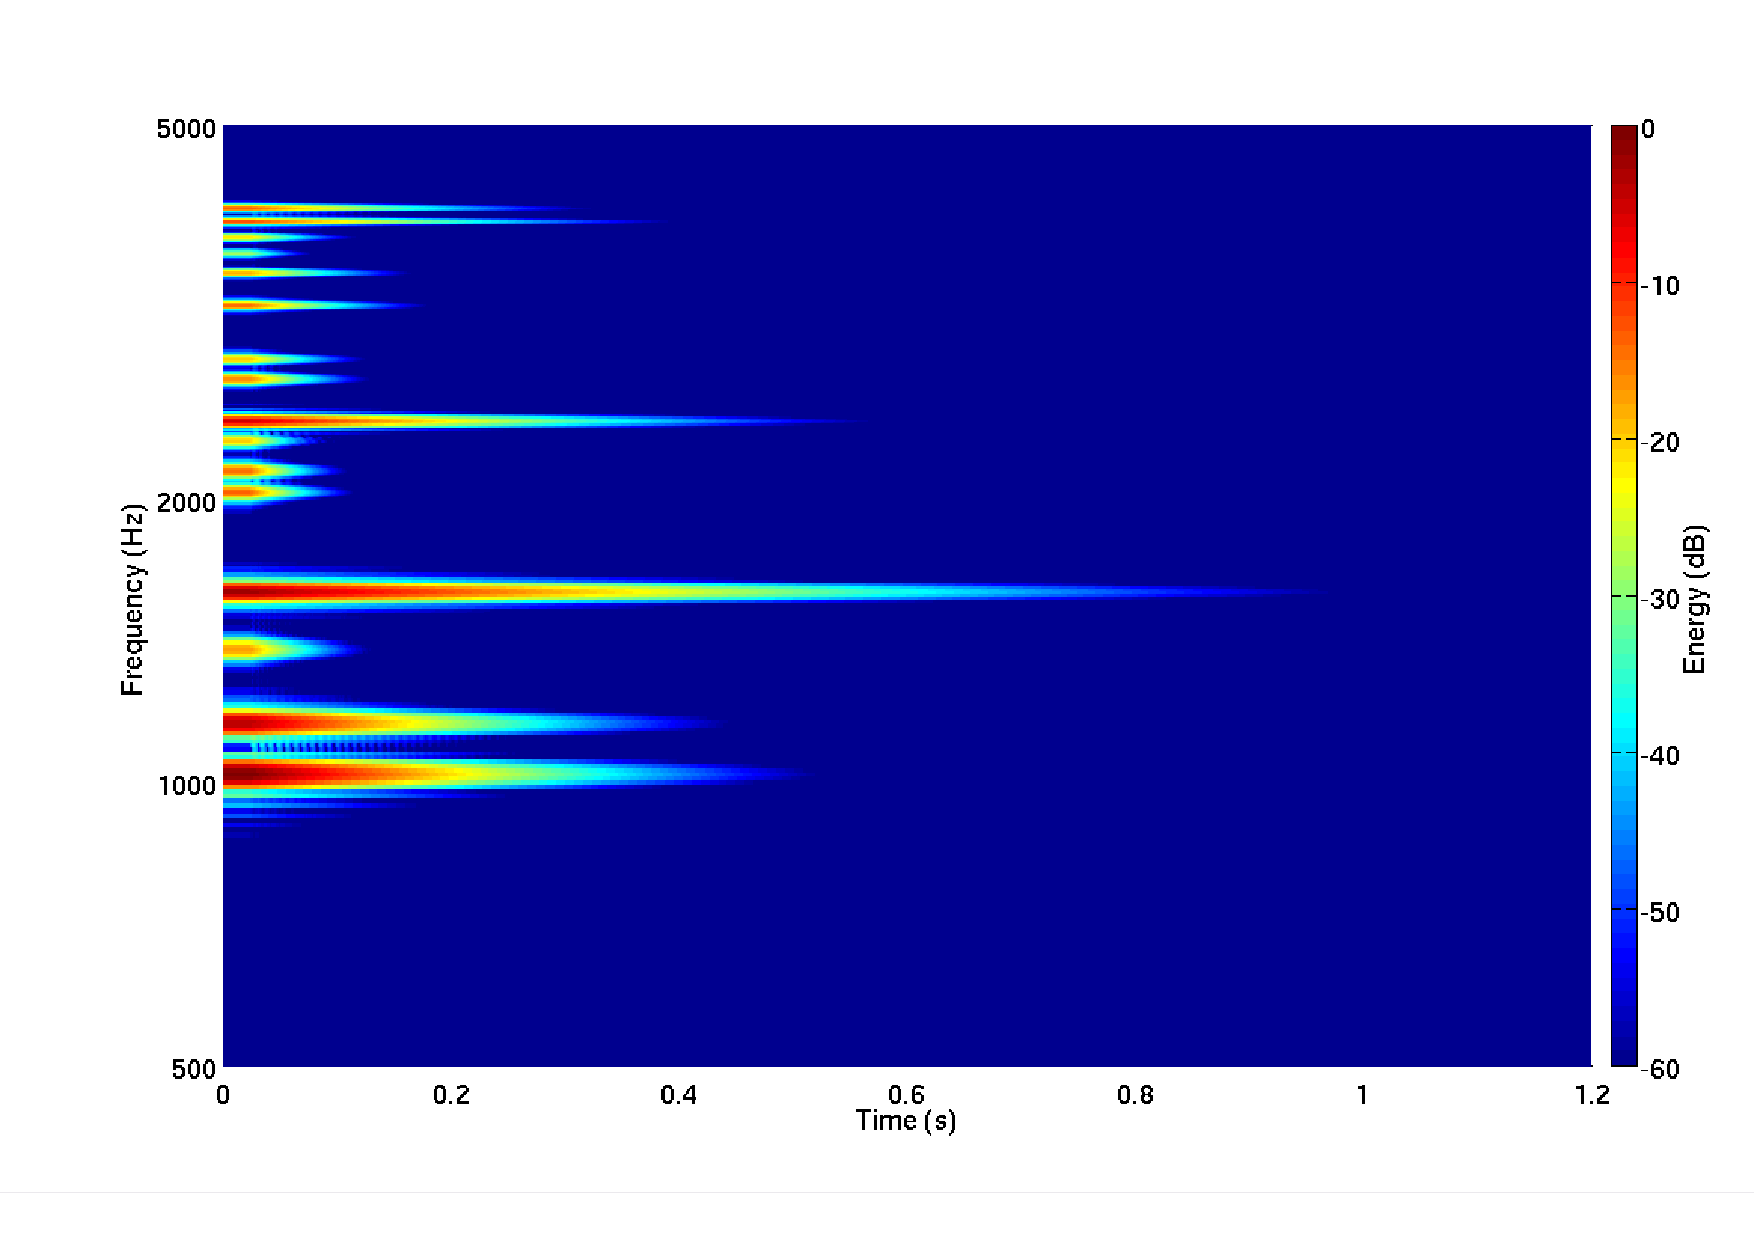
\includegraphics[width=\columnwidth]{pictures/canModalModel}
  \caption{Spectrogram of the output of the modal model generated with \texttt{ir2dsp.py} from a can IR}
  \label{fig:spectro2}
\end{figure}

\texttt{mesh2dsp.py} was tested with the geometric 3D model of a solid bar and provided good results. 

\section{Future Work}
\label{sec:future}

This work has been carried out as part of a larger project on designing a physical modeling toolkit for the \f{} programming language. \texttt{ir2dsp.py} and \texttt{mesh2dsp.py} will be integrated to it.

We plan to improve \texttt{ir2dsp.py} by using a better \textit{T60} measurement algorithm. Indeed, the \textit{T60} of each mode is currently computed by measuring its bandwidth after taking the FFT of the entire impulse response. A better approach would be to extract this information from a time-frequency representation of the signal (i.e., spectrogram), which would be more accurate.

Finally, we would like to try other open-source packages than Elmer to carry out the FEA in \texttt{mesh2dsp.py} to get better results and to smooth its integration in our \f{} physical modeling toolkit.  

\section{Conclusion}

We presented a series of tools allowing to design at very high level ready-to-use physical models of musical instruments. Models can be generated from impulse responses or 3D graphical representations of physical objects.

While the models generated by this system are far from being accurate, we believe that it provides a convenient way for composers and musicians to design expressive custom instruments usable in a musical context.  

% TODO: link to github

\section{Acknowledgements}

Our thanks go to Yann Orlarey for his help with the use of Faust.

\bibliographystyle{acl}
\bibliography{sample}

\end{document}
